% Printed 468; principal PDF 475; Google PDF 479.
\par\clearpage
\noindent\makebox[0pt][l]{\fontsize{13}{16}\selectfont 468}\hfill{\small\textbf{BRIEFWECHSEL.}}\hfill\null\par\medskip
\noindent erst nach ein paar Minuten eintreffen würde, und wenn man sich dann beeilt, abzulesen und die Alhidade vorzurücken, so gelingt es wohl, dass der Beobachter an dem Ort, wohin das Licht geworfen wird, über 2 Minuten den vollen Glanz geniesst. Offenbar ist die Mühe ohne Vergleich geringer, wenn sogleich am grossen Spiegel, senkrecht auf der Ebene des Sextanten, unter der Neigung $a$ ein dritter Spiegel befestigt ist. Der Sextant wird dadurch ein vollkommener Sonnenspiegel, und steht nur deswegen sehr nach, weil theils das kleine Fernrohr mit seinem halben Licht nicht auf sehr grosse Distanzen trägt, und theils, weil dieser dritte Spiegel bei den Bewegungen des Sextanten auf seinem Stativ nicht in Ruhe bleibt. Ich denke jedoch behuf der Contresignale an meinem Sextanten einen solchen dritten Spiegel anbringen zu lassen.

\par\noindent\hspace*{\parindent}Bei den kleinen bisher angestellten Versuchen ist es nun so gegangen: \textls[120]{Zuerst}, bloss auf der Terrasse der Sternwarte, Distanz 60 Meter, war das Licht so, dass man auch nicht einen Augenblick ohne Schmerz hinsehen durfte. \textls[120]{Zweitens} etwas abwärts, Distanz 150 Meter, war das nur ein paar Secunden fortgesetzte Hinsehen dem Auge peinlich. Nur diese beiden Versuche habe ich selbst gemacht, da ich bisher niemand habe, der die Stellung machen könnte, und also dies selbst thun musste. (Es würde besser sein, einen andern dazu abzurichten, wenn nicht das Stativ sehr unvollkommen balancirt wäre, so dass es, wenn die Versuche nicht völlig misslingen sollen, mit äusserst leichter Hand behandelt werden muss; wenn ein dritter Spiegel erst da ist, fällt offenbar diese Schwierigkeit weg.) Bei den folgenden Versuchen haben theils der jetzt hier angesetzte Professor \textsc{Ulrich}, theils Hr. Lieutenant \textsc{Hartmann} beobachtet.

\par\noindent\hspace*{\parindent}Beim \textls[120]{dritten} Versuch war die Distanz 300 Meter. Hr. Professor \textsc{Ulrich} beschrieb das Licht als herrlich und beim anhaltenden Hinsehen dem Auge beschwerlich.

\par\noindent\hspace*{\parindent}Vorgestern \textls[120]{ein vierter Versuch}, auf die Distanz 2000 Meter. Hr. Professor \textsc{Ulrich} qualificirte das Licht wieder als herrlich und verglich es mit einem 3-fachen Glanze der Venus, wie sie, wenn sie am schönsten ist, bei Nacht erscheint. Sein Begleiter habe nicht genug sein Erstaunen zu erkennen geben können, wie ein solcher Glanz hervorgebracht sei.

\par\noindent\hspace*{\parindent}Gestern \textls[120]{fünfter Versuch}, am Platz des künftig zu errichtenden \textls[120]{süd-}

% Printed 469; principal PDF 476; Google PDF 480.
\par\clearpage
\noindent\null\hfill{\small\textbf{HELIOTROP.}}\hfill\makebox[0pt][r]{\fontsize{13}{16}\selectfont 469}\par\medskip
\noindent\textls[120]{lichen} Meridianzeichens, wo ich eine beträchtliche Waldung habe durchhauen lassen müssen, Distanz 11890 Meter. Hr. Lieutenant \textsc{Hartmann} betitelt das Licht wieder als \textls[120]{herrlich} und meint, dass es an Intensität wohl noch der Venus in der Abenddämmerung gleich gekommen, aber für das Auge, wie er sich ausdrückte, \textls[120]{beleidigender} gewesen sei. Es versteht sich, dass alle diese Beobachtungen mit blossen Augen gemacht sind. Ein Arbeiter, den er bei sich hatte, habe beim ersten Aufblitzen erschrocken Feuer geschrien. Im Theodolithenfernrohr schien der Faden an der Stelle dieses scharfen Lichtpunkts völlig zerschnitten.

\par\noindent\hspace*{\parindent}Der Spiegel an meinem Sextanten hat genau 2 Pariser Zoll Breite und $1\frac14$ Zoll Höhe; der Spiegel des von \textsc{Rumpf} verfertigten Heliotrops hat nahe dieselben Dimensionen.

\par\noindent\hspace*{\parindent}Ich habe geglaubt, dass es Ihnen nicht unangenehm sein würde, diese Resultate zu erfahren. So lange, bis ich mit dem wirklichen Sonnenspiegel erst noch etwas mehr ins Grosse gehende Versuche angestellt habe, möchte ich nicht gern, dass auswärts etwas davon transpirte.

\par\noindent\hspace*{\parindent}Ich habe nun die beste Hoffnung, dass diese Vorrichtung auch in den grössten Distanzen meines Dreieckssystems aushelfen soll. Ich glaube, wenn man die Sonnenspiegel nach der zweiten in meinem letzten Briefe angedeuteten Einrichtung ausführt, und den Spiegel hinlänglich gross macht, so gibt es in Zukunft für die Grösse der Triangelseiten keine Grenzen mehr, als die die Kugelgestalt der Erde setzt.

\par\noindent\hspace*{\parindent}Vielleicht können diese Ideen auch in andern Beziehungen noch wichtige Anwendungen finden, z. B. als Signale für astronomische Längenbestimmungen, da man dies Licht immer ganz augenblicklich bedecken und wieder erscheinen lassen kann. Vielleicht selbst zu andern telegraphischen Signalisirungen, wenigstens zu Zeiten, wo die Sonne etwas anhaltend scheint, wenn den sehr genau zu messenden Intervallen des Erscheinens und Verschwindens verabredete Bedeutungen beigelegt werden.

\par\noindent\hspace*{\parindent}Mein Hohehagen-Signal ist gestern fertig geworden. Ich denke diese Woche noch (wenn \textsc{Rumpf} Wort hält) theils die schwierige Berichtigung des Sonnenspiegels, theils die Messung des Winkels Hohehagen-Meridianzeichen hier zu absolviren und dann nach dem Hohehagen abzugehen.\enspace .\ .\ .\ .\ .\ .

% Printed 470; principal PDF 477; Google PDF 481.
\par\clearpage
\noindent\makebox[0pt][l]{\fontsize{13}{16}\selectfont 470}\hfill{\small\textbf{BRIEFWECHSEL.}}\hfill\null\par\bigskip
\begin{center}{\large\textsc{Gauss} an \textsc{Schumacher}.\quad Göttingen, 11. Julius 1821.}\end{center}
\par\noindent\hspace*{\parindent}.\ .\ .\ .\ .\ .\enspace Vielleicht könnte eine Nachricht über mein neues Instrument, dem ich den Namen Heliotrop beilegen möchte, die Eröffnung[\textsuperscript{*})] machen: ich hoffe, dass diese Manier zu beobachten für die höhere Geodäsie von der grössten Wichtigkeit werden kann. Auf kurze Distanzen (bis 2 Meilen) können Sie sich keinen schönern Zielpunkt denken, als reflectirtes Licht von einer hellen Wolke; reflectirtes Sonnenlicht, hoffe ich, soll in den allergrössten Entfernungen das schönste Ziel darbieten.\enspace .\ .\ .\ .\ .\ .
\par\bigskip
\begin{center}{\large\textsc{Gauss} an \textsc{Schumacher}.\quad Göttingen, 8. November 1821.}\end{center}
\par\noindent\hspace*{\parindent}.\ .\ .\ .\ .\ .\enspace Den Artikel über den Heliotrop in den Göttingischen gelehrten Anzeigen hat \textsc{Zach} in seinem Journal[\textsuperscript{**})] übersetzt; es sind aber in der Übersetzung mehrere Unrichtigkeiten. Von den beiden neuen Heliotropen ist der eine jetzt fertig; er thut eine prachtvolle Wirkung, nur macht es uns grosse Schwierigkeit, gute Spiegel zu bekommen; die bisherigen sind äusserst schlecht, was zwar der Wirkung an sich wenig oder gar keinen Eintrag thut, aber die Berichtigung sehr erschwert. Gestern machte ich einen Versuch mit Mondlicht; in einer freilich nur kleinen Entfernung von etwa 250 Meter machte es einen überaus schönen Effect, das Licht dem der Venus (bei Nacht, wenn sie hoch steht) zwar ähnlich, aber vielfach brillanter. Das Telegraphiren habe ich ziemlich ausgebildet, ich kann allenfalls einige Tausend verschiedene Zeichen geben.\enspace .\ .\ .\ .\ .\ .
\par\bigskip
\begin{center}{\large\textsc{Gauss} an \textsc{Schumacher}.\quad Steinkrug am Deister, 10. Julius 1822.}\end{center}
\par\noindent\hspace*{\parindent}.\ .\ .\ .\ .\ .\enspace Ich habe dieses Jahr 3 wirkliche Heliotrope und noch einen andern Heliotropapparat in Thätigkeit; zwei von jenen spielen immer in der Ferne. Es ist eine Pracht (a luxury), in schönen Abendstunden Winkel zwischen zwei Heliotroplichtern zu messen, und die Harmonie der Resultate ist dann oft ganz zum Bewundern.\enspace .\ .\ .\ .\ .\ .
\par\medskip\noindent\rule{4cm}{.4pt}\par
\begingroup\footnotesize
\noindent\hspace*{\parindent}[\textsuperscript{*}) \textsc{Schumacher} hatte um einen Beitrag für die Astronomischen Nachrichten gebeten.]\par
\noindent\hspace*{\parindent}[\textsuperscript{**}) Correspondance astronomique, géographique, etc. du Baron \textsc{de Zach}.\quad V. Band.\quad 1821, S. 374/382.]\par
\endgroup

% Printed 471; principal PDF 478; Google PDF 482.
\par\clearpage
\noindent\null\hfill{\small\textbf{HELIOTROP.}}\hfill\makebox[0pt][r]{\fontsize{13}{16}\selectfont 471}\par\bigskip
\begin{center}{\large\textsc{Gauss} an \textsc{Schumacher}.\quad Göttingen, 15. Januar 1827.}\end{center}
\par\noindent\hspace*{\parindent}Hieneben erhalten Sie den Aufsatz über die Berichtigung der Heliotrope zurück[\textsuperscript{*})]. Nur bei dem $3^{\mathrm{ten}}$ Mittel zur $7^{\mathrm{ten}}$ Berichtigung ist, falls ich mich recht erinnere, meine Meinung eigentlich anders gewesen, als hier gesagt wird; ich meinte nemlich einen Sextanten so zu stellen, dass die Spiegel genau parallel sind, nemlich Index auf dem \textls[120]{wahren} Nullpunkt, und worauf es hier eigentlich ankommt, die Spiegel in Rücksicht auf ihre Verticalität zur Ebene des Sextanten gehörig berichtigt. Wenn man dann den Sextanten so hält, dass man das aus dem I. Spiegelbestandtheile reflectirte Bild eines hellen gut begrenzten Gegenstandes (besser als die Sonne würden die Fixsterne erster Grösse oder hinlänglich entferntes Heliotroplicht sein) direct, das aus dem II. Spiegelbestandtheile aber durch die Reflexion von den beiden Spiegeln des Sextanten, also im Grunde durch dreimalige Reflexion, sieht, so soll nur Ein Bild gesehen werden. Indessen gestehe ich, dass ich dies Mittel selbst nicht angewandt habe; auch ist die Brauchbarkeit von den Dimensionen des Heliotrops und Sextanten abhängig, nemlich die Entfernung der Mitten von I und II soll etwas kleiner sein, als die Entfernung der Mitte des grossen Sextantenspiegels von der Axe des Fernrohrs. Sie mögen also immerhin es so, wie es
\begin{center}
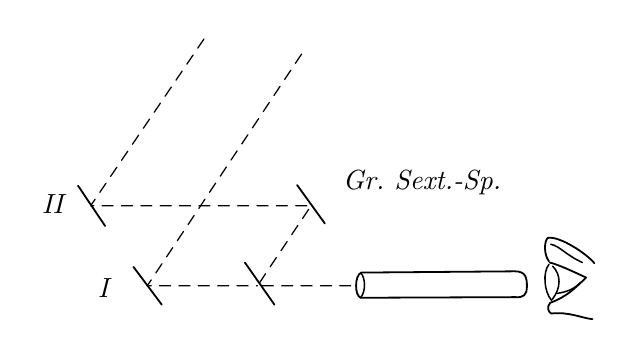
\begin{tikzpicture}[x=.008cm,y=-.008cm,line cap=round,line join=round]
\path[use as bounding box] (50,0) rectangle (970,475);
\draw[line width=.45pt,dash pattern=on 4pt off 3pt] (330,18)--(150,283)--(500,283)--(415,410)--(575,410);
\draw[line width=.45pt,dash pattern=on 4pt off 3pt] (485,42)--(240,410)--(415,410);
\draw[line width=.65pt] (130,251)--(173,315) (218,380)--(263,440) (478,250)--(522,311) (395,373)--(442,440);
\node[font=\itshape,anchor=east] at (122,280) {II};
\node[font=\itshape,anchor=east] at (194,414) {I};
\node[font=\itshape,anchor=west] at (535,247) {Gr.\ Sext.-Sp.};
\draw[line width=.65pt] (580,389)--(824,387)..controls (841,387) and (843,397)..(843,411)..controls (843,425) and (837,429)..(825,428)--(579,429)..controls (569,426) and (569,393)..(580,389);
\draw[line width=.55pt] (579,389)..controls (587,399) and (587,418)..(579,429);
\draw[line width=.65pt] (878,371)..controls (870,361) and (870,340)..(876,334)..controls (894,330) and (938,359)..(950,374);
\draw[line width=.55pt] (881,344)..controls (897,348) and (903,360)..(931,373);
\draw[line width=.65pt] (879,373)..controls (892,376) and (916,387)..(937,397)..controls (919,414) and (907,427)..(880,437)..controls (874,443) and (877,453)..(882,454)..controls (910,451) and (929,461)..(947,463);
\draw[line width=.55pt] (884,379)..controls (897,392) and (898,413)..(883,432);
\draw[line width=.55pt] (878,376)..controls (868,388) and (870,419)..(882,433);
\draw[line width=.55pt] (891,422)..controls (906,420) and (918,415)..(928,405);
\end{tikzpicture}
\end{center}
\noindent geschrieben ist, stehen lassen, zumal da jeder Leser sich die nöthigen Cautelen leicht hinzu denken kann, z. B. dass man am besten thut, das Spiegelsystem so zu stellen, dass die Sonne ungefähr in derjenigen Ebene ist, auf welcher die Spiegelaxe senkrecht ist; dass man, wenn zwischen den Messungen auf beiden Spiegelbestandtheilen einige Zeit verfliesst (mehr als einige Secunden, was jedoch von einem geschickten Beobachter wohl vermieden werden kann), darauf Rücksicht nehmen müsse.\enspace .\ .\ .\ .\ .\ .
\par\medskip\noindent\rule{4cm}{.4pt}\par
\begingroup\footnotesize\noindent\hspace*{\parindent}[\textsuperscript{*}) Siehe die folgende Abhandlung.]\par\endgroup
\begin{center}\rule{3.5cm}{.4pt}\end{center}

% Printed 472; principal PDF 479; Google PDF 483.
\par\clearpage
\noindent\makebox[0pt][l]{\fontsize{13}{16}\selectfont 472}\hfill{\small\textbf{HELIOTROP.}}\hfill\null\par
\vspace*{4.4cm}
\begin{center}
\begin{tabular}{c}\hline
\small\textbf{Astronomische Nachrichten, Bd. V, Nr. 116, Februar 1827, S. 329--334.}\\\hline
\end{tabular}\par\bigskip
{\large Die Berichtigung des Heliotrops.}
\end{center}
\par\noindent\hspace*{\parindent}Zur völligen Berichtigung des Heliotrops sind in allem acht Operationen erforderlich:
\par\noindent\hangindent=1.8em\hangafter=1\hspace*{1em}1.\ 2.\quad Die optische Axe des Fernrohrs wird durch die Correctionsschrauben $E$ und $F$ (Fig. 1) mit der Drehungsaxe desselben parallel gemacht.
\par\noindent\hangindent=1.8em\hangafter=1\hspace*{1em}3.\quad Die Spiegelaxe $AB$ stellt man durch die Schrauben $CC$ (Fig. 1) an dem einen Arme der Gabel, welche jene Axe trägt, auf die Drehungsaxe des Fernrohrs senkrecht.
\par\noindent\hangindent=1.8em\hangafter=1\hspace*{1em}4.\ 5.\ 6.\quad Die Ebenen der drei Spiegel (des kleinern und der beiden Bestandtheile des grössern) werden durch die Schrauben $G$, $H$, $I$ (Fig. 2) der Spiegelaxe parallel gestellt.
\par\noindent\hangindent=1.8em\hangafter=1\hspace*{1em}7.\quad Durch die Schraube $K$ (Fig. 2) wird der Bestandtheil II des grössern Spiegels in eine mit dem Bestandtheil I parallele Ebene gebracht.
\par\noindent\hangindent=1.8em\hangafter=1\hspace*{1em}8.\quad Der kleine Spiegel muss durch die Schraube am Schwanze desselben so gestellt werden, dass die Ebene des Spiegels auf den Ebenen der beiden Bestandtheile des grossen senkrecht steht.
\par\noindent\hspace*{\parindent}Die Berichtigungen 1 und 2 übergehe ich als allgemein bekannt.

\par\noindent\hspace*{\parindent}Um die Berichtigung 3 auf eine ganz selbstständige Art auszuführen, stelle ich den Heliotrop auf ein festes Postament, richte die Spiegelaxe $AB$ (Fig. 3) vertical mit dem Stiele $AD$ nach unten, und drehe diesen Stiel, bis er nach der Ocularseite\textsuperscript{*}) hin mit der Fernrohraxe parallel ist. Alles bloss nach dem Augenmaass. An dem Stiel $AD$ hänge ich eine nicht zu empfind-
\par\medskip\noindent\rule{4cm}{.4pt}\par
\begingroup\footnotesize\noindent\hspace*{\parindent}\textsuperscript{*}) Dies kann auch, mutatis mutandis, umgekehrt gehalten werden.\par\endgroup

% Printed 473; principal PDF 480; Google PDF 484.
\par\clearpage
\noindent\null\hfill{\small\textbf{HELIOTROP.}}\hfill\makebox[0pt][r]{\fontsize{13}{16}\selectfont 473}\par\medskip
\noindent liche Libelle, und bringe durch Änderung der Länge der Drähte, woran sie aufgehangen ist, die Blase \textls[120]{nahe} und nachher durch die Fussschrauben \textls[120]{genau} zum Einstehen. Hierauf drehe ich den Stiel um $180^\circ$ um die Spiegelaxe, hebe das Fernrohr vorsichtig aus, und lege es in der entgegengesetzten Lage wieder ein (Fig. 4). Die Berichtigung ist unnöthig, wenn die Blase dann wieder einsteht; sonst wird die eine Hälfte des Ausschlags an den Fussschrauben, und die andere an den Schrauben $CC$ (Fig. 1) corrigirt. Eine Restitution in die vorige Lage zeigt, ob die Vertheilung richtig gemacht ist. Die bei diesem Verfahren nöthigen Cautelen übergehe ich, da jeder sie auch ohne Anleitung finden wird, und ich das Verfahren späterhin entweder gar nicht oder nur zur ersten groben Berichtigung angewandt habe\textsuperscript{*}).

\par\noindent\hspace*{\parindent}Ein Verfahren, welches ich für die Berichtigungen 4, 5 und 6 angewandt habe, beruht auf dem Princip, dass eine Ebene $ab$ (Fig. 5) durch eine halbe Umdrehung um eine ihr parallele Axe $AB$ in eine mit ihrer ersten Lage $ab$ parallele, aber entgegengesetzte Lage $cd$ gebracht wird. Sind die Axe und die Ebene aber nicht parallel, wie in Fig. 6, so werden die beiden Lagen $ab$ und $cd$ auch nicht parallel sein. Um dies an einem Spiegel zu prüfen, stelle ich zwei mit Kreuzfäden versehene Fernrohre $M$, $N$ (Fig. 7) so auf, dass deutliche Objecte $O$, $P$ auf ihren optischen Axen erscheinen, und dass letztere sich nahe schneiden, oder nahe in einer Ebene liegen. Den zu prüfenden Spiegel stelle ich, nachdem ich die Gabel vom Fernrohre abgenommen und auf einem Kästchen oder Brett befestigt habe, auf einen Tisch nahe in den Schnitt der optischen Axen, so dass die Drehungsaxe $AB$ ungefähr in ihrer Ebene liegt und den Winkel derselben bisecirt. Ich stelle dann den Spiegel $L$ perpendiculär auf jene Ebene und bewirke durch kleine Drehungen und sanfte Anschläge sowohl an den Spiegel selbst als an das Kästchen, dass das Bild von $O$, aus dem Spiegel reflectirt, auf der optischen Axe von $M$ erscheine. Darauf drehe ich den Spiegel um $180^\circ$ um seine Axe und sehe nach, ob in dieser Lage (Fig. 8) das Bild von $P$ auf der optischen Axe von $N$ erscheint. Kann dies nicht durch blosse Drehung des Spiegels um die Axe $AB$ erreicht werden, so muss die Hälfte an dem Kästchen und die
\par\medskip\noindent\rule{4cm}{.4pt}\par
\begingroup\footnotesize\noindent\hspace*{\parindent}\textsuperscript{*}) Übrigens beruht die Brauchbarkeit dieser Methode darauf\rlap{\hspace{.05em}\raisebox{2ex}{.}}, dass die cylindrischen Ansätze, mit welchen das Fernrohr in den Lagern ruht, genau gleiche Dicke haben, auf welchen Umstand bei den von Hrn. \textsc{Rumpf} verfertigten Instrumenten sorgfältig Rücksicht genommen ist.\par\endgroup
\par\medskip\noindent\makebox[0pt][l]{\small IX.}\makebox[.86\linewidth][r]{60}\par

% Printed 474; principal PDF 481; Google PDF 485.
\par\clearpage
\noindent\makebox[0pt][l]{\fontsize{13}{16}\selectfont 474}\hfill{\small\textbf{HELIOTROP.}}\hfill\null\par\medskip
\noindent andere Hälfte an der Lage des Spiegels gegen seine Axe corrigirt werden. Die Objecte $O$, $P$ brauchen, insofern der Spiegel hart an seiner Axe sitzt, nicht weit entfernt zu sein; ich habe sie in eine Entfernung von etwa 70--80 Fuss gestellt.

\par\noindent\hspace*{\parindent}Zur Erreichung der Berichtigung 7 lassen sich mancherlei Mittel anwenden. Das einfachste, und welches auch hinreichende Genauigkeit gewährt, ist, eine gerade Linie, mit der die Spiegelaxe ungefähr parallel ist, in den beiden Hälften des grossen Spiegels zu betrachten, worin sie als eine gerade Linie erscheinen muss, was das blosse Auge schon mit grosser Genauigkeit beurtheilt.\ \raisebox{.55ex}{.}\ Ich habe dazu die Façade der Sternwarte gebraucht. --- Ein zweites Mittel ist: ein feines Object (Heliotroplicht) mit einem Fernrohr von grossem Objectiv (Cometensucher) in beiden Spiegeln zugleich zu sehen, und an dem Bestandtheile II zu corrigiren, bis man nur ein Bild hat. Offenbar wird hiedurch auch die Correction 6 erhalten, wenn 5 schon gemacht ist. --- Ein drittes Mittel ist: von den beiden Bestandtheilen des grossen Spiegels als künstliche Horizonte die Sonnenhöhen mit einem Sextanten zu nehmen, die, wenn die Berichtigung gemacht ist, sich gleich sein müssen. --- Ein viertes Mittel wird sich sogleich darbieten.

\par\noindent\hspace*{\parindent}Um die $8^{\mathrm{te}}$ Berichtigung zu machen, habe ich folgendes Verfahren am besten gefunden. Ich stelle den Heliotrop und ein Hülfsfernrohr mit Kreuzfäden so auf, dass die optische Axe des letztern mit der des Heliotropfernrohrs parallel ist, und etwa um die Hälfte der Entfernung der Mitten der beiden Bestandtheile des grossen Spiegels in derselben Verticalebene höher liegt (Fig. 9). Dies bewirke ich dadurch, dass ich den Heliotrop auf ein gut zu sehendes entferntes Object richte, das Fernrohr herausnehme, und nachdem das Hülfsfernrohr in der angegebenen Höhe auf dasselbe Object gerichtet ist, in umgekehrter Lage wieder einlege. Die Spiegelaxe wird darauf senkrecht gestellt, mit dem Bestandtheile I nach oben, und durch Drehung des Spiegelsystems und nöthigenfalls auch des Fernrohrs bewirkt, dass ein Object durch Reflexion aus dem kleinen Spiegel auf der optischen Axe des Heliotropfernrohrs erscheine. Erscheint dasselbe Object durch Reflexion aus dem Bestandtheile I des grossen Spiegels auf der optischen Axe des Hülfsfernrohrs, so macht die Ebene des kleinen Spiegels mit dem des Bestandtheils I einen rechten Winkel; sonst wird das Fehlende an der Schwanzschraube corri-

% Printed 475; principal PDF 482; Google PDF 486.
\par\clearpage
\noindent\null\hfill{\small\textbf{HELIOTROP.}}\hfill\makebox[0pt][r]{\fontsize{13}{16}\selectfont 475}\par\medskip
\noindent girt. Die Berichtigung 7 kann hierauf auch auf dieselbe Weise geprüft werden, indem man das Heliotropfernrohr $180^\circ$ um seine Axe dreht, dass der Bestandtheil II oben kommt, wobei aber offenbar Objecte auf der andern Seite genommen werden müssen.

\par\noindent\hspace*{\parindent}Die bisher angeführten Methoden sind alle von einander unabhängig, bloss mit der Einschränkung, dass 7 nach 6 gemacht werden muss, weil eine Berührung der Schraube $I$ die Berichtigung 7 afficiren würde. Zur Berichtigung 3 aber, insofern 4 schon gemacht ist, oder zu beiden zugleich, habe ich ein Verfahren angewandt, was auf dem Princip beruht, dass eine Fläche, die um eine auf ihr senkrechte Axe gedreht wird, immer in derselben Ebene bleibt. Wird daher der kleine Spiegel senkrecht auf die Axe des Heliotropfernrohrs gestellt (welches auf doppelte Weise geschehen kann, indem nemlich die reflectirende Fläche dem Fernrohr \textls[120]{zu-} oder davon \textls[120]{abgewandt} wird), so muss das Bild eines jeden Objects in diesem Spiegel ruhen, während das Fernrohr um seine Axe gedreht wird. Ich stelle demnach den kleinen Spiegel, zuerst nach dem Augenmaasse, senkrecht auf die Fernrohraxe, die reflectirende Fläche abwärts vom Objective (Fig. 10), und bewirke dies genauer, indem ich zuerst mit blossen Augen beurtheile, ob das Bild eines seitwärts liegenden Gegenstandes durch Drehung des Fernrohrs um seine Axe unbeweglich bleibt. Hierauf stelle ich, indem die Spiegelaxe vertical steht, ein Hülfsfernrohr mit Kreuzfäden so auf, dass das aus dem kleinen Spiegel reflectirte Bild irgend eines seitwärts liegenden Gegenstandes auf der optischen Axe desselben erscheint, und zwar so, dass diese Axe nahe auf die Mitte des kleinen Spiegels gerichtet ist. Ich drehe jetzt das Heliotropfernrohr halb um seine Axe herum und sehe zu, ob das reflectirte Bild auf der optischen Axe des Hülfsfernrohrs geblieben ist. Die Hälfte der Abweichung links oder rechts wird sonst durch Drehung des Spiegelsystems, die Hälfte der Abweichung nach oben oder unten aber an den Schrauben $CC$ (Fig. 1) corrigirt, und das Hülfsfernrohr\textsuperscript{*}) wieder so gerichtet, dass das reflectirte Bild genau auf der optischen Axe erscheint. Eine abermalige halbe Umdrehung des Heliotropfernrohrs um seine Axe wird dann zeigen, ob die Vertheilung richtig gemacht ist. Die Ebene des kleinen Spiegels $ab$ (Fig. 11) steht also jetzt genau senkrecht auf der Fernrohraxe;
\par\medskip\noindent\rule{4cm}{.4pt}\par
\begingroup\footnotesize\noindent\hspace*{\parindent}\textsuperscript{*}) Oder der Heliotrop, welches aber ohne Gehülfen nicht bequem geschehen kann.\par\endgroup
\par\medskip\noindent\makebox[.86\linewidth][r]{60\textsuperscript{*}}\par

% Printed 476; principal PDF 483; Google PDF 487.
\par\clearpage
\noindent\makebox[0pt][l]{\fontsize{13}{16}\selectfont 476}\hfill{\small\textbf{HELIOTROP.}}\hfill\null\par\medskip
\noindent mithin ist, wenn die Berichtigung 4 schon gemacht ist, auch 3 vollkommen. Ist aber die Ebene des kleinen Spiegels nicht mit der Axe $AB$ (Fig. 11) parallel, so wird er durch Drehung des Spiegelsystems nicht in eine auf der Fernrohraxe senkrechte aber entgegengesetzte Lage gebracht werden können, sondern bei der grössten Abweichung um die doppelte Neigung gegen die Spiegelaxe davon abstehen (Fig. 12). Man wiederhole also in dieser Lage das vorige Experiment, wobei aber das Object in einer Richtung liegen muss, die mit der Fernrohraxe einen stumpfen Winkel bildet (Fig. 13). Ist der Spiegel nun so gestellt, dass das reflectirte Bild, welches zuerst bei der senkrechten Lage der Spiegelaxe auf der optischen Axe erschien, nach einer halben Umdrehung um die Fernrohraxe weder rechts noch links erscheint, so sind in dem Falle, dass es auch weder höher noch tiefer liegt, die Berichtigungen 3 und 4 beide vollkommen; sonst wird von dem Unterschiede $\frac14$ an der Schraube $CC$ (Fig. 1) und $\frac14$ an der Schraube $G$ corrigirt. Das Hülfsfernrohr wird dann wieder auf das reflectirte Bild gestellt, und nach einer halben Umdrehung des Heliotropfernrohrs um seine Axe zur Prüfung nachgesehen, ob das Bild auf der optischen Axe geblieben ist. Wenn noch etwas nachzuhelfen ist, so ist es gut, die Prüfung in der ersten Lage des Spiegels zu wiederholen. Die Objecte brauchen hiezu nicht entfernt zu sein, wenn nur das Fadensystem des Hülfsfernrohrs dieser Entfernung gemäss gestellt ist.
\par\vspace{2.5cm}\begin{center}\rule{3.5cm}{.4pt}\end{center}

% Printed 477; principal PDF 484; Google PDF 488.
\par\clearpage
\noindent\null\hfill{\small\textbf{HELIOTROP.}}\hfill\makebox[0pt][r]{\fontsize{13}{16}\selectfont 477}\par\bigskip
\begin{center}
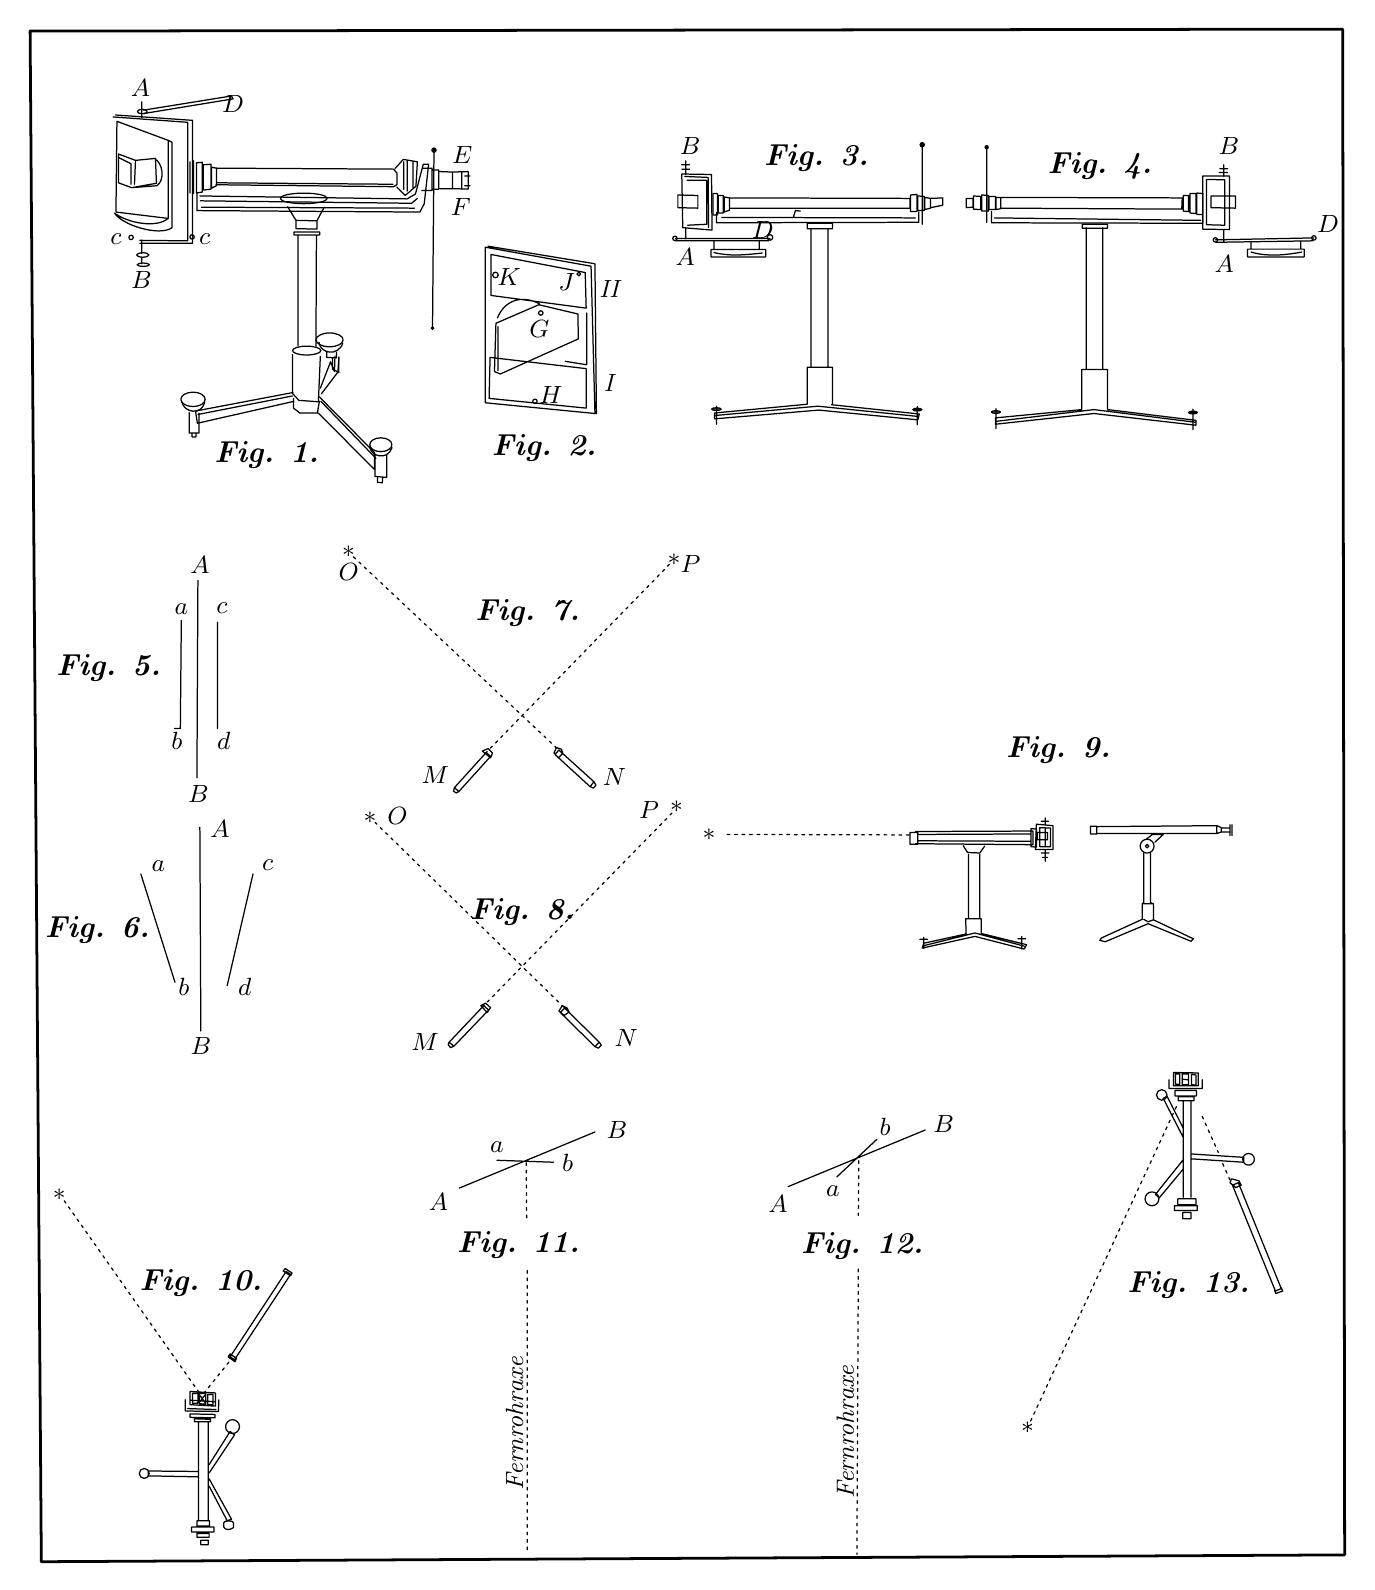
\begin{tikzpicture}[x=.0062cm,y=-.0062cm,line cap=round,line join=round,line width=.45pt,
  every node/.style={font=\fontsize{9}{10}\selectfont\itshape,inner sep=0pt},
  ray/.style={line width=.45pt,dash pattern=on 1pt off 1.7pt},
  caption/.style={font=\fontsize{11}{12}\selectfont\bfseries\itshape}]
\path[use as bounding box] (30,415) rectangle (2735,3560);
\draw[line width=1pt] (35,422)--(2726,418)--(2730,3546)--(58,3560)--cycle;
% Figures 1 and 2: perspective instrument and its mirror system.
\begin{scope}[shift={(110,500)}]
\draw (95,98)--(248,109)--(248,352)--(150,351)
 (100,94)--(258,105)--(258,357)--(150,357)
 (103,107)--(208,146)--(208,306)--(101,293)--cycle;
\draw (98,295)..controls (112,319) and (190,344)..(216,325)--(216,150)--(208,146)
 (98,295)..controls (123,315) and (184,327)..(208,306);
\draw (106,174)--(141,187)--(182,183)--(184,234)--(133,243)--(106,233)--cycle
 (141,187)--(139,236) (106,181)--(132,194)--(132,236)
 (181,184)..controls (197,193) and (202,227)..(185,239)--(133,243);
\draw (154,67)--(154,100) (158,84)--(338,55)--(341,61)--(158,91)
 (154,351)--(154,378) (154,387)--(154,399);
\draw (155,87) ellipse[x radius=1.8pt,y radius=.8pt]
 (156,381) ellipse[x radius=2.2pt,y radius=.8pt]
 (157,401) ellipse[x radius=2.2pt,y radius=.6pt];
\draw (132,345) circle[radius=.8pt] (257,344) circle[radius=.8pt];
\node at (151,39) {$A$}; \node at (341,72) {$D$}; \node at (153,432) {$B$};
\node at (101,348) {$c$}; \node at (283,349) {$c$};
\draw (253,190)--(253,254) (260,188)--(260,255)
 (266,192)--(278,191)--(278,252)--(266,254)--cycle
 (280,196)--(296,195)--(296,246)--(280,248)--cycle
 (297,201)--(307,203)--(307,239)--(297,244)--cycle;
\draw (307,203)--(670,205)--(677,213)--(677,237)--(670,241)--(306,237)
 (308,233)--(669,236)
 (673,204)--(690,185)--(719,190)--(716,240)--(694,259)--(677,242)
 (691,190)--(691,247) (698,188)--(698,250) (710,190)--(710,243);
\draw (273,260)--(698,266)--(715,256)--(731,195)--(742,195)--(733,276)--(724,293)--(267,290)--(267,254)
 (274,270)--(707,275)--(719,265) (276,283)--(713,285)
 (731,203)--(749,203)--(749,249)--(728,249)
 (750,207)--(763,207)--(763,246)--(750,246)
 (765,210)--(791,211)--(791,245)--(765,245)
 (791,211)--(823,210)--(823,246)--(791,245)
 (810,211)--(810,246) (816,219)--(827,219) (816,239)--(827,239);
\draw (753,167)--(750,531);
\fill (753,166) circle[radius=1pt] (750,531) circle[radius=.7pt];
\node at (811,177) {$E$}; \node at (808,282) {$F$};
\draw (486,265) ellipse[x radius=8.5pt,y radius=1.9pt];
\draw (453,282)--(470,310)--(513,311)--(528,283)
 (470,310)--(470,327)--(513,328)--(513,311)
 (466,334)--(519,334)--(519,340)--(466,340)--cycle
 (474,341)--(474,567) (512,342)--(511,568)
 (463,585)--(463,665)--(476,679)--(516,682)--(520,589);
\draw (492,577) ellipse[x radius=5.1pt,y radius=1.6pt];
\draw (465,675)--(465,695)--(478,705)--(514,705)--(518,681)
 (464,663)--(264,701)--(268,726)--(466,681)
 (269,708)--(463,670)
 (518,672)--(631,786)--(631,821)--(516,705)
 (521,681)--(634,798)
 (520,654)--(541,600)--(549,620)--(550,588)
 (522,666)--(556,621)--(558,591);
\draw (259,677) ellipse[x radius=4.4pt,y radius=2.6pt]
 (539,555) ellipse[x radius=4.9pt,y radius=2.5pt]
 (644,770) ellipse[x radius=4pt,y radius=2.5pt];
\draw (236,682)..controls (240,704) and (276,711)..(283,683)
 (251,704)--(251,746)--(271,746)--(271,705)
 (257,746)--(257,754)--(265,754)--(265,747)
 (517,560)..controls (520,583) and (556,590)..(566,562)
 (533,580)--(533,591)--(553,592)--(553,581)
 (545,592)--(545,615)--(558,622)--(558,590)
 (621,773)..controls (623,795) and (658,803)..(667,776)
 (632,790)--(632,835)--(656,837)--(656,791)
 (637,836)--(637,847)--(647,848)--(648,836);
\node[caption] at (410,790) {Fig. 1.};
\draw (858,365)--(1075,404)--(1083,706)--(858,684)--cycle
 (864,363)--(1083,399)--(1086,706)--(1083,706)
 (870,380)--(1063,417)--(1065,490)--(870,464)--cycle
 (868,591)--(1065,614)--(1065,695)--(866,675)--cycle
 (880,521)--(968,483)--(1048,502)--(1049,553)--(889,625)--(877,620)--cycle
 (884,528)--(884,618)
 (883,510)..controls (901,468) and (939,465)..(969,481)
 (1066,500)--(1066,606)--(1022,599);
\draw (879,422) circle[radius=1pt] (1050,420) circle[radius=.7pt]
 (972,500) circle[radius=.8pt] (960,681) circle[radius=.8pt];
\node at (907,427) {$K$}; \node at (1025,437) {$J$};
\node at (969,533) {$G$}; \node at (993,669) {$H$};
\node at (1112,450) {II}; \node at (1111,644) {I};
\node[caption] at (979,776) {Fig. 2.};
\end{scope}
% Figures 3 and 4: the two separately drawn positions with hanging level.
\begin{scope}[shift={(1310,600)}]
\draw (61,115)--(122,116)--(123,230)--(63,225)--cycle
 (67,120)--(115,122)--(116,225) (72,128)--(112,128)--(112,218)--(73,220)
 (53,158)--(94,159)--(94,185)--(53,184)--cycle
 (69,88)--(69,116) (61,96)--(77,96) (61,105)--(77,105)
 (69,225)--(69,248) (48,247)--(242,247) (48,252)--(239,252);
\draw (47,247) circle[radius=.8pt] (242,245) circle[radius=1pt];
\draw (127,252)--(127,270) (220,253)--(220,269)
 (121,270)--(233,270)--(233,285)--(121,285)--cycle
 (127,276)..controls (159,284) and (190,281)..(226,277);
\node at (68,285) {$A$}; \node at (78,57) {$B$}; \node at (227,230) {$D$};
\draw (125,155)--(134,155)--(134,199)--(125,199)--cycle
 (136,159)--(146,159)--(146,195)--(136,195)--cycle
 (148,162)--(159,164)--(159,189)--(148,193)--cycle
 (159,164)--(529,165)--(529,185)--(159,185)
 (132,194)--(132,215)--(547,214)--(547,193)
 (143,204)--(540,205) (290,203)--(294,190)--(304,191)
 (530,158)--(543,157)--(543,192)--(530,192)--cycle
 (545,160)--(558,161)--(558,190)--(545,190)--cycle
 (559,163)--(571,165)--(571,185)--(559,188)--cycle
 (571,165)--(596,164)--(596,179)--(571,184)
 (554,55)--(554,218);
\fill (554,55) circle[radius=1pt];
\draw (318,216)--(370,216)--(370,227)--(318,227)--cycle
 (326,227)--(326,510) (361,227)--(361,510)
 (318,511)--(370,511)--(370,588)
 (318,511)--(318,587)--(128,605)--(128,617)--(342,599)--(545,619)--(548,607)--(368,588)
 (130,610)--(340,591)--(545,612)
 (132,591)--(132,628) (123,597)--(141,597)
 (544,592)--(544,629) (535,598)--(553,598);
\draw (132,597) ellipse[x radius=1.7pt,y radius=.5pt]
 (544,598) ellipse[x radius=1.6pt,y radius=.5pt];
\node[caption] at (337,83) {Fig. 3.};
\draw (644,165)--(658,165)--(658,183)--(644,184)--cycle
 (659,160)--(674,161)--(674,188)--(659,187)--cycle
 (676,158)--(690,159)--(690,191)--(676,191)--cycle
 (691,161)--(704,161)--(704,188)--(691,188)--cycle
 (705,163)--(715,163)--(715,186)--(705,188)--cycle
 (715,163)--(1087,164)--(1086,187)--(715,185)
 (1089,159)--(1100,159)--(1100,192)--(1089,191)--cycle
 (1103,155)--(1115,155)--(1115,196)--(1103,195)--cycle
 (1117,154)--(1129,155)--(1129,198)--(1117,198)--cycle
 (702,205)--(1125,210) (696,192)--(696,215)--(1129,216)--(1129,200)
 (686,60)--(686,214);
\fill (686,60) circle[radius=.8pt];
\draw (1129,119)--(1184,119)--(1184,229)--(1129,228)--cycle
 (1137,126)--(1174,127)--(1174,220)--(1137,219)--cycle
 (1146,160)--(1196,160)--(1196,185)--(1146,184)--cycle
 (1172,96)--(1172,120) (1164,104)--(1180,104) (1163,112)--(1180,112)
 (1172,230)--(1172,253) (1155,250)--(1357,246) (1156,255)--(1355,252);
\draw (1155,250) circle[radius=.8pt] (1357,246) circle[radius=.8pt];
\draw (1228,254)--(1228,269) (1330,253)--(1330,269)
 (1221,269)--(1337,269)--(1337,285)--(1221,285)--cycle
 (1228,275)..controls (1265,286) and (1305,280)..(1332,275);
\node at (1173,300) {$A$}; \node at (1183,57) {$B$}; \node at (1386,217) {$D$};
\draw (882,218)--(934,218)--(934,226)--(882,226)--cycle
 (890,225)--(890,515) (924,225)--(924,515)
 (881,516)--(934,516)--(934,598)
 (881,516)--(881,598)--(704,615)--(704,628)--(906,606)--(1115,630)--(1115,620)--(934,598)
 (706,622)--(906,598)--(1114,624)
 (705,596)--(705,637) (696,603)--(714,603)
 (1109,597)--(1109,639) (1100,604)--(1118,604);
\draw (705,603) ellipse[x radius=1.6pt,y radius=.5pt]
 (1109,604) ellipse[x radius=1.6pt,y radius=.5pt];
\node[caption] at (918,98) {Fig. 4.};
\end{scope}
% Figures 5 and 6: finite, unequal line segments without arrows.
\begin{scope}[shift={(70,1470)}]
\draw (309,78)--(307,483) (275,160)--(273,382)--(261,382) (349,164)--(349,382);
\node at (313,47) {$A$}; \node at (310,516) {$B$};
\node at (275,137) {$a$}; \node at (266,408) {$b$};
\node at (358,135) {$c$}; \node at (362,408) {$d$};
\node[caption] at (126,257) {Fig. 5.};
\draw (313,584)--(315,1002) (192,680)--(262,902) (422,680)--(369,909);
\node at (354,587) {$A$}; \node at (315,1033) {$B$};
\node at (228,663) {$a$}; \node at (280,912) {$b$};
\node at (452,661) {$c$}; \node at (405,912) {$d$};
\node[caption] at (103,795) {Fig. 6.};
\end{scope}
% Figures 7 and 8: crossing rays and two separate telescopes in each figure.
\begin{scope}[shift={(650,1450)}]
\node at (38,40) {$\ast$}; \node at (705,55) {$\ast$};
\node at (38,80) {$O$}; \node at (739,64) {$P$};
\draw[ray] (48,50)--(469,446) (696,65)--(320,451);
\draw (255,523)--(320,451)--(329,459)--(264,531)--cycle
 (312,448)--(324,443)--(333,452)--(329,462)--cycle
 (255,523)--(253,530)--(258,534)--(264,531)
 (469,446)--(541,511)--(533,521)--(461,455)--cycle
 (464,441)--(474,444)--(477,453)--(468,462)--(459,452)--cycle
 (541,511)--(545,518)--(540,524)--(533,521);
\node at (216,497) {$M$}; \node at (583,501) {$N$};
\node[caption] at (405,165) {Fig. 7.};
\node at (82,584) {$\ast$}; \node at (710,563) {$\ast$};
\node at (138,582) {$O$}; \node at (654,568) {$P$};
\draw[ray] (92,594)--(481,975) (701,575)--(315,970);
\draw (244,1045)--(315,970)--(325,979)--(254,1053)--cycle
 (309,970)--(319,965)--(329,974)--(322,984)--cycle
 (244,1045)--(242,1050)--(247,1056)--(254,1053)
 (481,975)--(552,1045)--(543,1054)--(472,984)--cycle
 (476,970)--(486,975)--(490,983)--(480,990)--(469,981)--cycle
 (552,1045)--(556,1051)--(550,1057)--(543,1054);
\node at (195,1044) {$M$}; \node at (607,1036) {$N$};
\node[caption] at (394,778) {Fig. 8.};
\end{scope}
% Figure 9: heliotrop and auxiliary telescope, separately elevated.
\begin{scope}[shift={(1380,1820)}]
\node at (47,250) {$\ast$}; \draw[ray] (84,249)--(459,250);
\draw (459,245)--(475,245)--(475,269)--(459,269)--cycle
 (470,243)--(711,242)--(711,270)--(470,268)
 (477,249)--(705,248) (477,262)--(705,263)
 (707,237)--(718,238)--(718,275)--(707,274)--cycle
 (718,228)--(752,231)--(752,280)--(716,280)--cycle
 (725,235)--(747,236)--(747,274)--(725,274)--cycle
 (736,237)--(736,272) (720,245)--(741,245)--(741,260)--(720,260)--cycle
 (736,215)--(736,229) (728,222)--(743,222)
 (736,280)--(736,304) (728,287)--(744,287) (731,296)--(741,296);
\draw (568,272)--(577,286)--(602,287)--(612,273)
 (579,290)--(579,422) (602,290)--(602,422)
 (573,422)--(605,422)--(605,452)--(698,475)--(693,484)--(592,458)--(484,482)--(487,472)--(574,453)--cycle
 (487,477)--(592,451)--(693,478)
 (487,460)--(487,483) (479,464)--(495,464)
 (688,458)--(688,484) (680,463)--(696,463);
\draw (829,232)--(842,232)--(842,248)--(829,248)--cycle
 (841,233)--(1088,231)--(1088,247)--(841,247)
 (1088,231)--(1097,235)--(1097,244)--(1088,247)
 (1097,236)--(1115,236)--(1115,244)--(1097,244)
 (1115,229)--(1115,251) (1119,229)--(1119,251)
 (961,265)--(978,249)--(956,249)--(943,259);
\draw (945,273) circle[radius=2.5pt] (945,273) circle[radius=.65pt];
\draw (938,287)--(938,389)--(935,391)--(935,423)--(852,461)--(848,466)--(859,469)--(947,432)--(1035,468)--(1040,463)--(958,424)--(958,391)--(952,389)--(952,287)
 (935,391)--(958,391) (938,423)--(947,428)--(958,424);
\node[caption] at (763,76) {Fig. 9.};
\end{scope}
% Figure 10: end-on instrument, oblique auxiliary telescope and ray.
\begin{scope}[shift={(55,2710)}]
\node at (40,98) {$\ast$};
\draw[ray] (50,110)--(332,511) (336,505)--(393,434);
\draw (390,430)--(505,255)--(514,261)--(399,436)--cycle
 (499,254)--(503,249)--(517,258)--(514,264)--cycle
 (386,430)--(390,424)--(403,433)--(400,440)--cycle;
\draw (308,501)--(360,504)--(360,531)--(308,528)--cycle
 (313,505)--(324,505)--(324,525)--(313,525)--cycle
 (327,505)--(340,505)--(340,527)--(327,526)--cycle
 (344,507)--(355,507)--(355,528)--(344,528)--cycle
 (327,508)--(339,524) (339,508)--(327,523)
 (309,519)--(360,522)
 (298,518)--(298,541)--(366,542)--(367,518)
 (303,536)--(361,538) (308,547)--(359,548)--(359,555)--(308,554)--cycle
 (317,557)--(350,558)--(350,563)--(317,563)--cycle
 (325,563)--(325,765) (345,563)--(345,764);
\draw (325,665)--(222,664)--(222,674)--(325,676)
 (347,651)--(390,583)--(399,590)--(347,668)
 (347,695)--(384,766)--(393,763)--(347,680);
\draw (214,669) circle[radius=1.8pt] (395,573) circle[radius=2.5pt];
\draw (377,770)..controls (377,765) and (397,765)..(397,770)--(397,780)..controls (389,786) and (380,785)..(377,779)--cycle
 (322,766)--(348,766)--(348,777)--(322,777)--cycle
 (311,779)--(357,779)--(357,789)--(311,789)--cycle
 (322,792)--(347,792)--(347,800)--(322,800)--cycle
 (330,806)--(345,806)--(345,815)--(330,815)--cycle;
\node[caption] at (330,278) {Fig. 10.};
\end{scope}
% Figures 11 and 12: the unlike inclinations are retained.
\begin{scope}[shift={(790,2630)}]
\draw (125,164)--(403,49) (202,107)--(318,111);
\node at (82,192) {$A$}; \node at (448,44) {$B$};
\node at (202,80) {$a$}; \node at (347,112) {$b$};
\draw[ray] (262,112)--(263,229) (264,333)--(264,915);
\node[caption] at (246,280) {Fig. 11.};
\node[rotate=90] at (238,647) {Fernrohraxe};
\draw (799,161)--(1080,45) (899,141)--(981,64);
\node at (778,196) {$A$}; \node at (1118,33) {$B$};
\node at (891,170) {$a$}; \node at (998,38) {$b$};
\draw[ray] (944,108)--(943,220) (943,330)--(940,915);
\node[caption] at (951,282) {Fig. 12.};
\node[rotate=90] at (916,664) {Fernrohraxe};
\end{scope}
% Figure 13: reverse position, its own oblique ray and auxiliary telescope.
\begin{scope}[shift={(2000,2490)}]
\draw[ray] (385,137)--(80,795) (438,157)--(471,231) (480,254)--(497,292);
\node at (80,796) {$\ast$};
\draw (370,82)--(370,100)--(438,100)--(438,82)
 (379,67)--(430,68)--(430,94)--(379,94)--cycle
 (383,70)--(392,70)--(392,91)--(383,91)--cycle
 (397,70)--(410,70)--(410,92)--(397,92)--cycle
 (397,81)--(410,82)
 (416,71)--(425,72)--(425,93)--(416,92)--cycle
 (382,104)--(426,104)--(426,115)--(382,115)--cycle
 (389,117)--(421,117)--(421,125)--(389,125)--cycle
 (399,125)--(399,323) (415,125)--(415,323)
 (399,200)--(358,120)--(366,116)--(399,181)
 (415,234)--(523,241)--(523,251)--(415,244)
 (399,246)--(342,317)--(350,324)--(399,265);
\draw (355,113) circle[radius=1.9pt] (533,245) circle[radius=2.1pt]
 (335,326) circle[radius=2.5pt];
\draw (388,326)--(425,326)--(425,338)--(388,338)--cycle
 (381,340)--(428,340)--(428,350)--(381,350)--cycle
 (398,354)--(415,354)--(415,367)--(398,367)--cycle
 (500,298)--(588,515)--(600,510)--(512,293)--cycle
 (495,293)--(498,285)--(513,289)--(518,298)--(507,303)--cycle
 (586,513)--(589,520)--(603,515)--(600,508);
\node[caption] at (410,502) {Fig. 13.};
\end{scope}
\end{tikzpicture}
\end{center}
